%%%%%%%%%%%%%%%%%%%%%%%%%%%%%%%%%%%%%%%%%%%%%%%%%%%%%%%%%%%%%%%%%%%%%%%%%%%%
% AGUtmpl.tex: this template file is for articles formatted with LaTeX2e,
% Modified December 2018
%
% This template includes commands and instructions
% given in the order necessary to produce a final output that will
% satisfy AGU requirements.
%
% FOR FIGURES, DO NOT USE \psfrag
%
%%%%%%%%%%%%%%%%%%%%%%%%%%%%%%%%%%%%%%%%%%%%%%%%%%%%%%%%%%%%%%%%%%%%%%%%%%%%
%
% IMPORTANT NOTE:
%
% SUPPORTING INFORMATION DOCUMENTATION IS NOT COPYEDITED BEFORE PUBLICATION.
%
%
%
%%%%%%%%%%%%%%%%%%%%%%%%%%%%%%%%%%%%%%%%%%%%%%%%%%%%%%%%%%%%%%%%%%%%%%%%%%%%
%
% Step 1: Set the \documentclass
%
%
% PLEASE USE THE DRAFT OPTION TO SUBMIT YOUR PAPERS.
% The draft option produces double spaced output.
%
% Choose the journal abbreviation for the journal you are
% submitting to:

% jgrga JOURNAL OF GEOPHYSICAL RESEARCH (use for all of them)
% gbc   GLOBAL BIOCHEMICAL CYCLES
% grl   GEOPHYSICAL RESEARCH LETTERS
% pal   PALEOCEANOGRAPHY
% ras   RADIO SCIENCE
% rog   REVIEWS OF GEOPHYSICS
% tec   TECTONICS
% wrr   WATER RESOURCES RESEARCH
% gc    GEOCHEMISTRY, GEOPHYSICS, GEOSYSTEMS
% sw    SPACE WEATHER
% ms    JAMES
% ef    EARTH'S FUTURE
%
%
%
% (If you are submitting to a journal other than jgrga,
% substitute the initials of the journal for "jgrga" below.)

\documentclass[draft,jgrga]{agutexSI2019}

%%%%%%%%%%%%%%%%%%%%%%%%%%%%%%%%%%%%%%%%%%%%%%%%%%%%%%%%%%%%%%%%%%%%%%%%%
%
%  SUPPORTING INFORMATION TEMPLATE
%
%% ------------------------------------------------------------------------ %%
%
%
%Please use this template when formatting and submitting your Supporting Information.

%This template serves as both a “table of contents” for the supporting information for your article and as a summary of files.
%
%
%OVERVIEW
%
%Please note that all supporting information will be peer reviewed with your manuscript. It will not be copyedited if the paper is accepted.
%In general, the purpose of the supporting information is to enable authors to provide and archive auxiliary information such as data tables, method information, figures, video, or computer software, in digital formats so that other scientists can use it.
%The key criteria are that the data:
% 1. supplement the main scientific conclusions of the paper but are not essential to the conclusions (with the exception of
%    including %data so the experiment can be reproducible);
% 2. are likely to be usable or used by other scientists working in the field;
% 3. are described with sufficient precision that other scientists can understand them, and
% 4. are not exe files.
%
%USING THIS TEMPLATE
%
%***All references should be included in the reference list of the main paper so that they can be indexed, linked, and counted as citations.  The reference section does not count toward length limits.
%
%All Supporting text and figures should be included in this document. Insert supporting information content into each appropriate section of the template. To add additional captions, simply copy and paste each sample as needed.

%Tables may be included, but can also be uploaded separately, especially if they are larger than 1 page, or if necessary for retaining table formatting. Data sets, large tables, movie files, and audio files should be uploaded separately. Include their captions in this document and list the file name with the caption. You will be prompted to upload these files on the Upload Files tab during the submission process, using file type “Supporting Information (SI)”

%IMPORTANT NOTE ON FIGURES AND TABLES
% Placeholders for figures and tables appear after the \end{article} command, after references.
% DO NOT USE \psfrag or \subfigure commands.
%
 \usepackage{graphicx}
%
%  Uncomment the following command to allow illustrations to print
%   when using Draft:
 \setkeys{Gin}{draft=false}
%
% You may need to use one of these options for graphicx depending on the driver program you are using. 
%
% [xdvi], [dvipdf], [dvipsone], [dviwindo], [emtex], [dviwin],
% [pctexps],  [pctexwin],  [pctexhp],  [pctex32], [truetex], [tcidvi],
% [oztex], [textures]
%
%
%% ------------------------------------------------------------------------ %%
%
%  ENTER PREAMBLE
%
%% ------------------------------------------------------------------------ %%

% Author names in capital letters:
%\authorrunninghead{BALES ET AL.}

% Shorter version of title entered in capital letters:
%\titlerunninghead{SHORT TITLE}

%Corresponding author mailing address and e-mail address:
%\authoraddr{Corresponding author: A. B. Smith,
%Department of Hydrology and Water Resources, University of
%Arizona, Harshbarger Building 11, Tucson, AZ 85721, USA.
%(a.b.smith@hwr.arizona.edu)}
\newcommand{\markred}[1]{\textcolor{red}{#1}}
%\newcommand{\markcyan}[1]{\textcolor{cyan}{#1}}
\newcommand{\markblue}[1]{\textcolor{blue}{#1}}
%\newcommand{\markgreen}[1]{\textcolor{magenta}{#1}}


\begin{document}

%% ------------------------------------------------------------------------ %%
%
%  TITLE
%
%% ------------------------------------------------------------------------ %%

%\includegraphics{agu_pubart-white_reduced.eps}


\title{Supporting Information for "Local lydraulic conductivity in heterogeneous porous media"}
%
% e.g., \title{Supporting Information for "Terrestrial ring current:
% Origin, formation, and decay $\alpha\beta\Gamma\Delta$"}
%
%DOI: 10.1002/%insert paper number here%

%% ------------------------------------------------------------------------ %%
%
%  AUTHORS AND AFFILIATIONS
%
%% ------------------------------------------------------------------------ %%


% List authors by first name or initial followed by last name and
% separated by commas. Use \affil{} to number affiliations, and
% \thanks{} for author notes.
% Additional author notes should be indicated with \thanks{} (for
% example, for current addresses).

% Example: \authors{A. B. Author\affil{1}\thanks{Current address, Antartica}, B. C. Author\affil{2,3}, and D. E.
% Author\affil{3,4}\thanks{Also funded by Monsanto.}}


\authors{Quirine Krol \affil{1}, Itzhak Fouxon \affil{1,2}, Pascal Corso \affil{1}, Markus Holzner \affil{1,2,3,4}}



% \affiliation{1}{First Affiliation}
% \affiliation{2}{Second Affiliation}
% \affiliation{3}{Third Affiliation}
% \affiliation{4}{Fourth Affiliation}

\affiliation{1}{ETH Zurich, Stefano Franscini-Platz 5, 8093 Zurich, Switzerland}
\affiliation{2}{Department of Computational Science and Engineering, Yonsei University, Seoul 120-749, South Korea}
\affiliation{3}{Swiss Federal Institute for Water Science and Technology EAWAG}
\affiliation{4}{Swiss Federal Institute for Forest, Snow and Landscape Research WSL}
%(repeat as many times as is necessary)





%% ------------------------------------------------------------------------ %%
%
%  BEGIN ARTICLE
%
%% ------------------------------------------------------------------------ %%

% The body of the article must start with a \begin{article} command
%
% \end{article} must follow the references section, before the figures
%  and tables.

\begin{article}

%% ------------------------------------------------------------------------ %%
%
%  TEXT
%
%% ------------------------------------------------------------------------ %%



\noindent\textbf{Contents of this file}
%%%Remove or add items as needed%%%
\begin{enumerate}
\item Direct numerical simulation of Stokes flow in porous media.
\item Pseudo code: Measuring local hydrualic conductivity.
\item Measuring the Transversal and Longitunidinal Energy Dissipation tensor.
%if Tables are larger than 1 page, upload as separate excel file
\end{enumerate}
\noindent\textbf{Additional Supporting Information (Files uploaded separately)}
\begin{enumerate}
\item Isopressure surfaces video
\item Pore identification video
\end{enumerate}

\noindent\textbf{Introduction}
%Type or paste your text here. The introduction gives a brief overview of the supporting information. You should include information %about as many of the following as possible (when appropriate):
% 1. a general overview of the kind of data files;
% 2. information about when and how the data were collected or created;
% 3. a general description of processing steps used;
% 4. any known imperfections or anomalies in the data.

%\clearpage

%Delete all unused file types below. Copy/paste for multiples of each file type as needed.
Below we describe the necessary steps and specific settings of the analysis presented in methodology. The fist part consists of the description of the direct numerical simulations performed that are used as a numerical experiment. In the second part we describe the details of the extraction of iso pressure surfaces and fluxes from which the hydraulic conductivity is calculated and integrated along consecutive pores. In the last part we take three samples from the three porous media to test the hypothesis that is made in Eq.() of the main article. 

\noindent\textbf{Geometry of the porous media interface}
For all 3 media we have used a levelset of a Gaussian Random Field given by a spectral density as given in \cite{roberts_transport_1995} The level-set was chosen such that we have porosity values of $0.68,0.34$ and $0.16$, for porous media 1, 2 and 3 respectively. For the third porous media we have chosen the level set value as high such that 

\noindent\textbf{Direct Numerical Simulations}

These porous media are used as input for direct numerical simulations (OpenFOAM v. 4.1) \citeA{weller_tensorial_1998}  that solves the Navier-Stokes equations in the pore space. The boundary conditions are defined at the inlet $p_1$ and outlet $p_2$ and a no-slip for the porous media-fluid interface. A visualization of the three porous media an the result of the DNS is visualized in Fig.~\ref{fig:DNS}
\begin{itemize}
	\item Three geometries generated by gaussian random fields, with porosity, specific surface area, Euler characteristic of 
	\item DNS employed with boundary conditions at the inlet and outlet defined by $delta p$. A no slip boundary condition is enforced on the domain walls as well as the porous media interface. 
	\item Result of the DNS gives estimated Re numbers by 

	\begin{equation}
		Re = u/s\eta
	\end{equation}

	\item Residuals were standard, check $10^{-6}$ took about 8 hours using 32 cores using the Euler cluster. 


\end{itemize}

\begin{figure}[htbp!]\label{fig:segmentation}
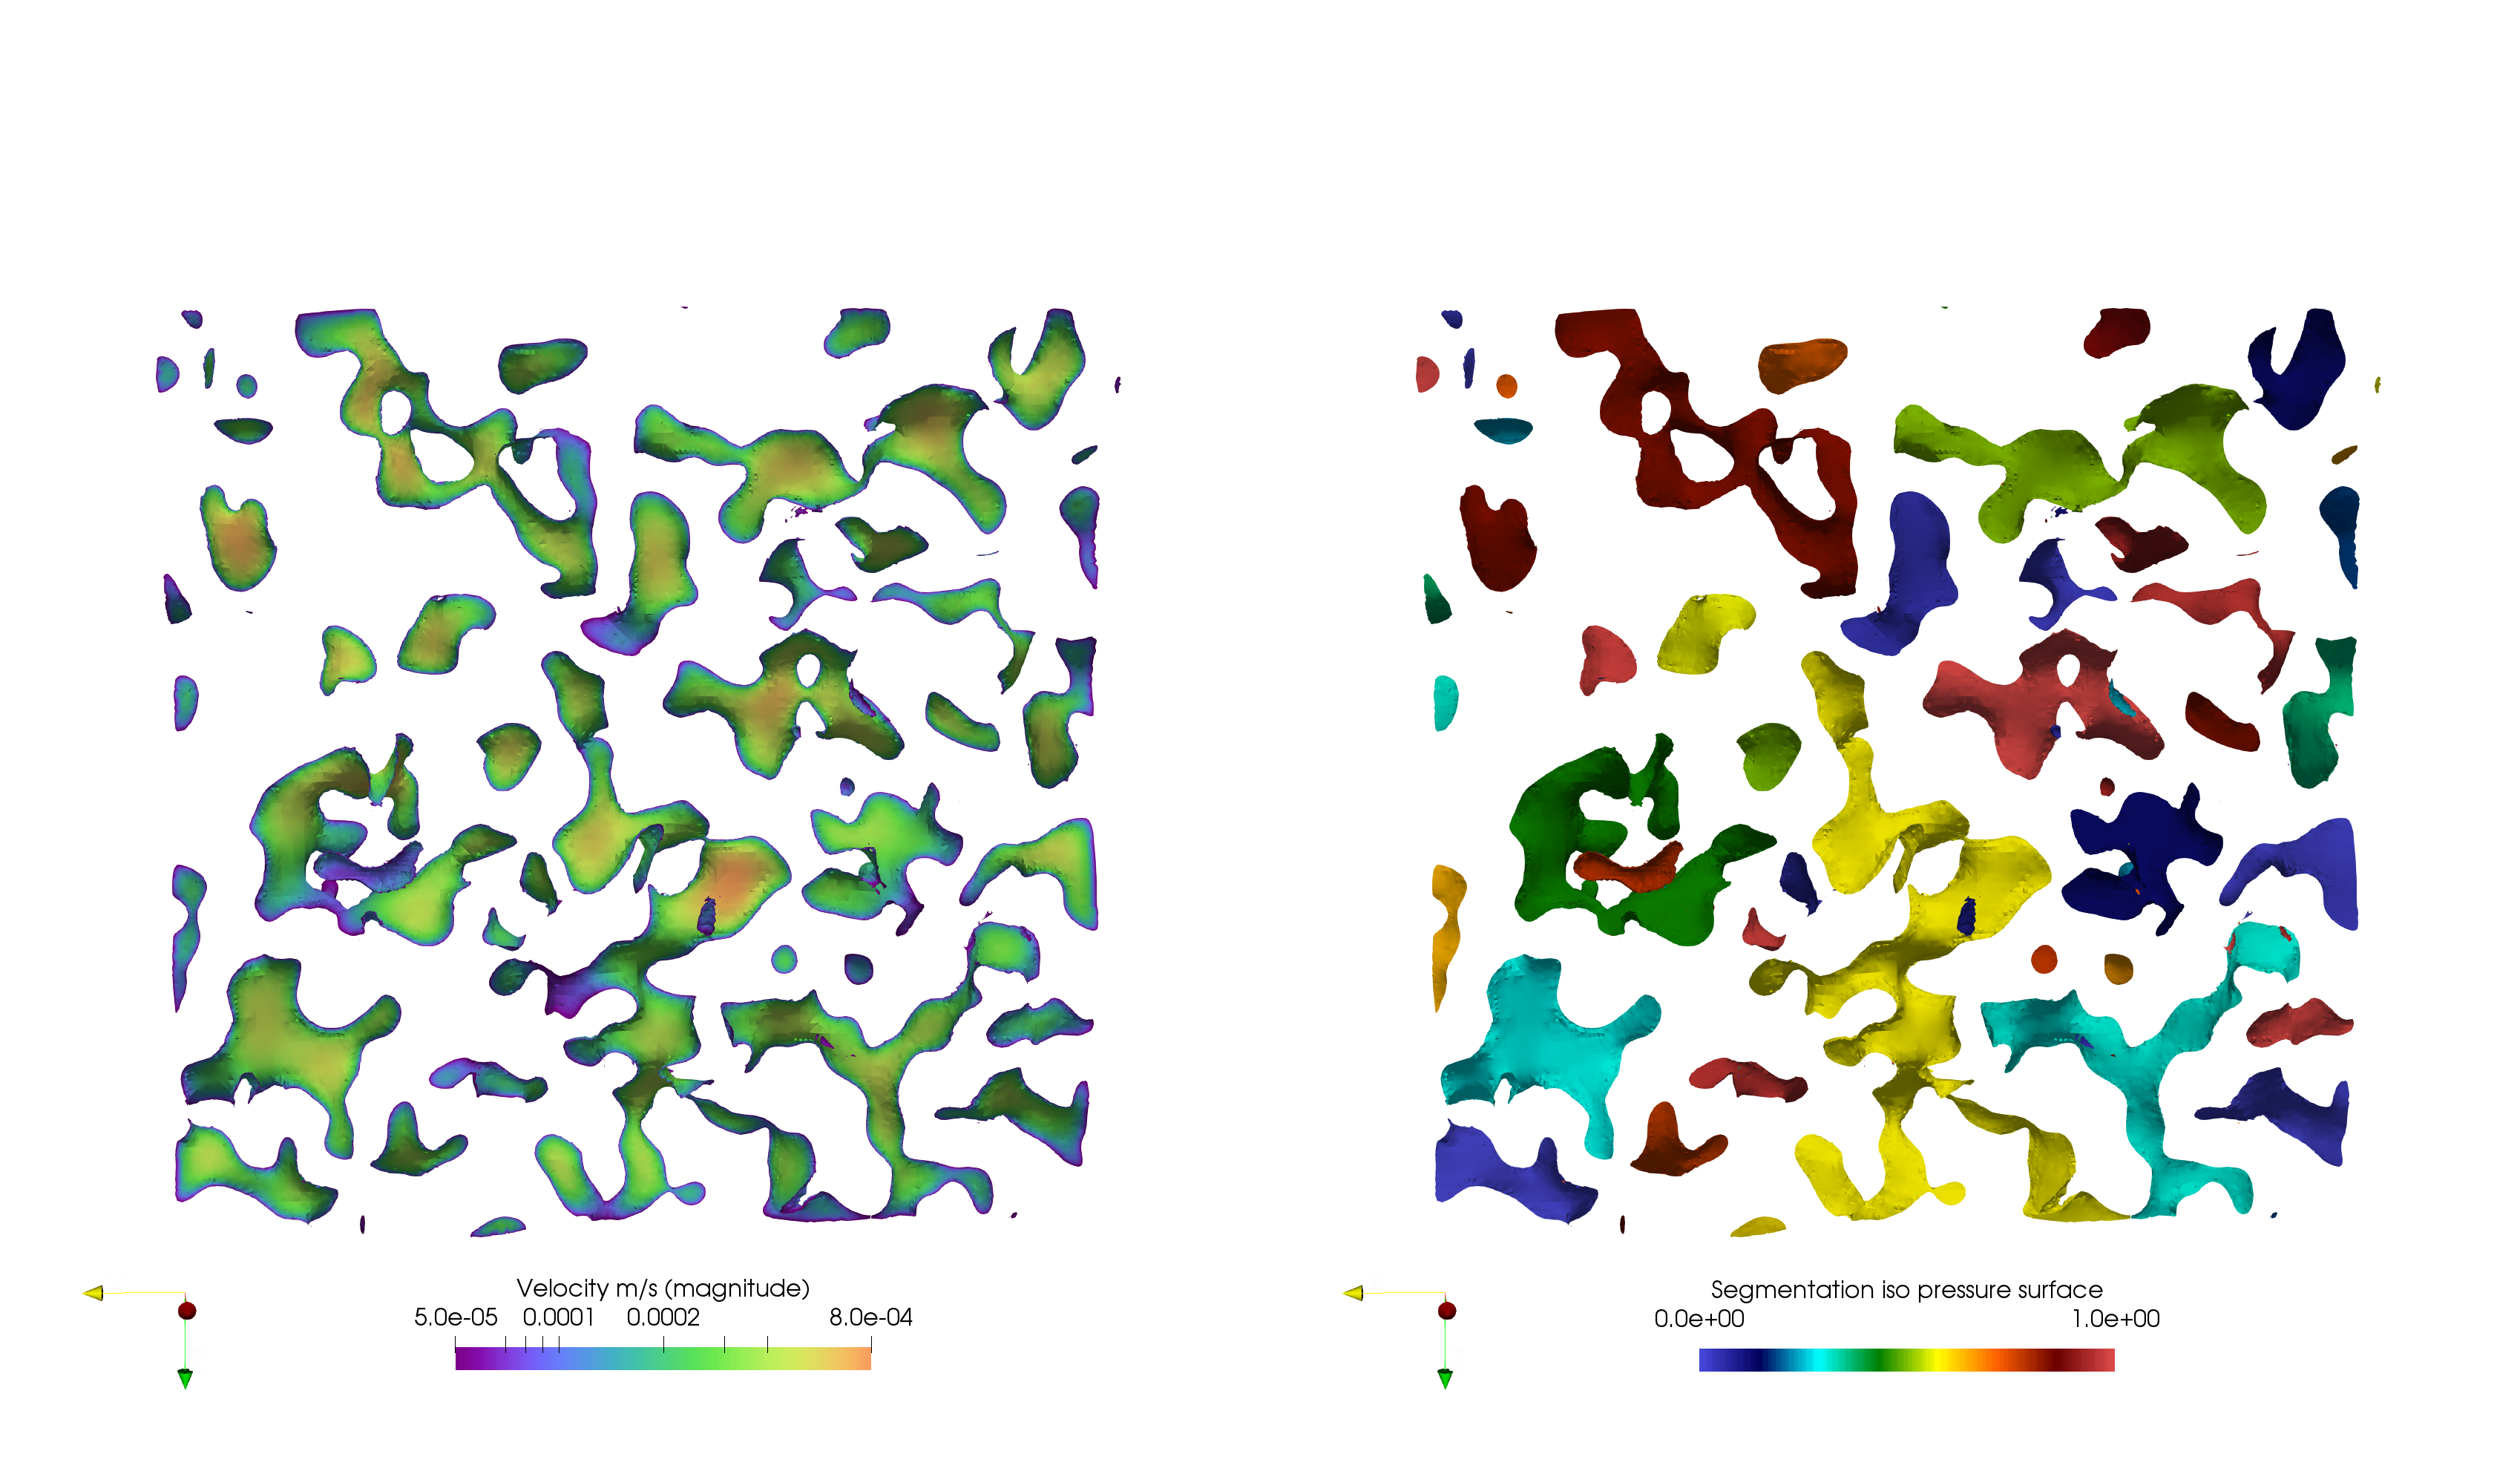
\includegraphics[height=6cm]{figures/semgentation_veloctiy_iso_p_surface.png}
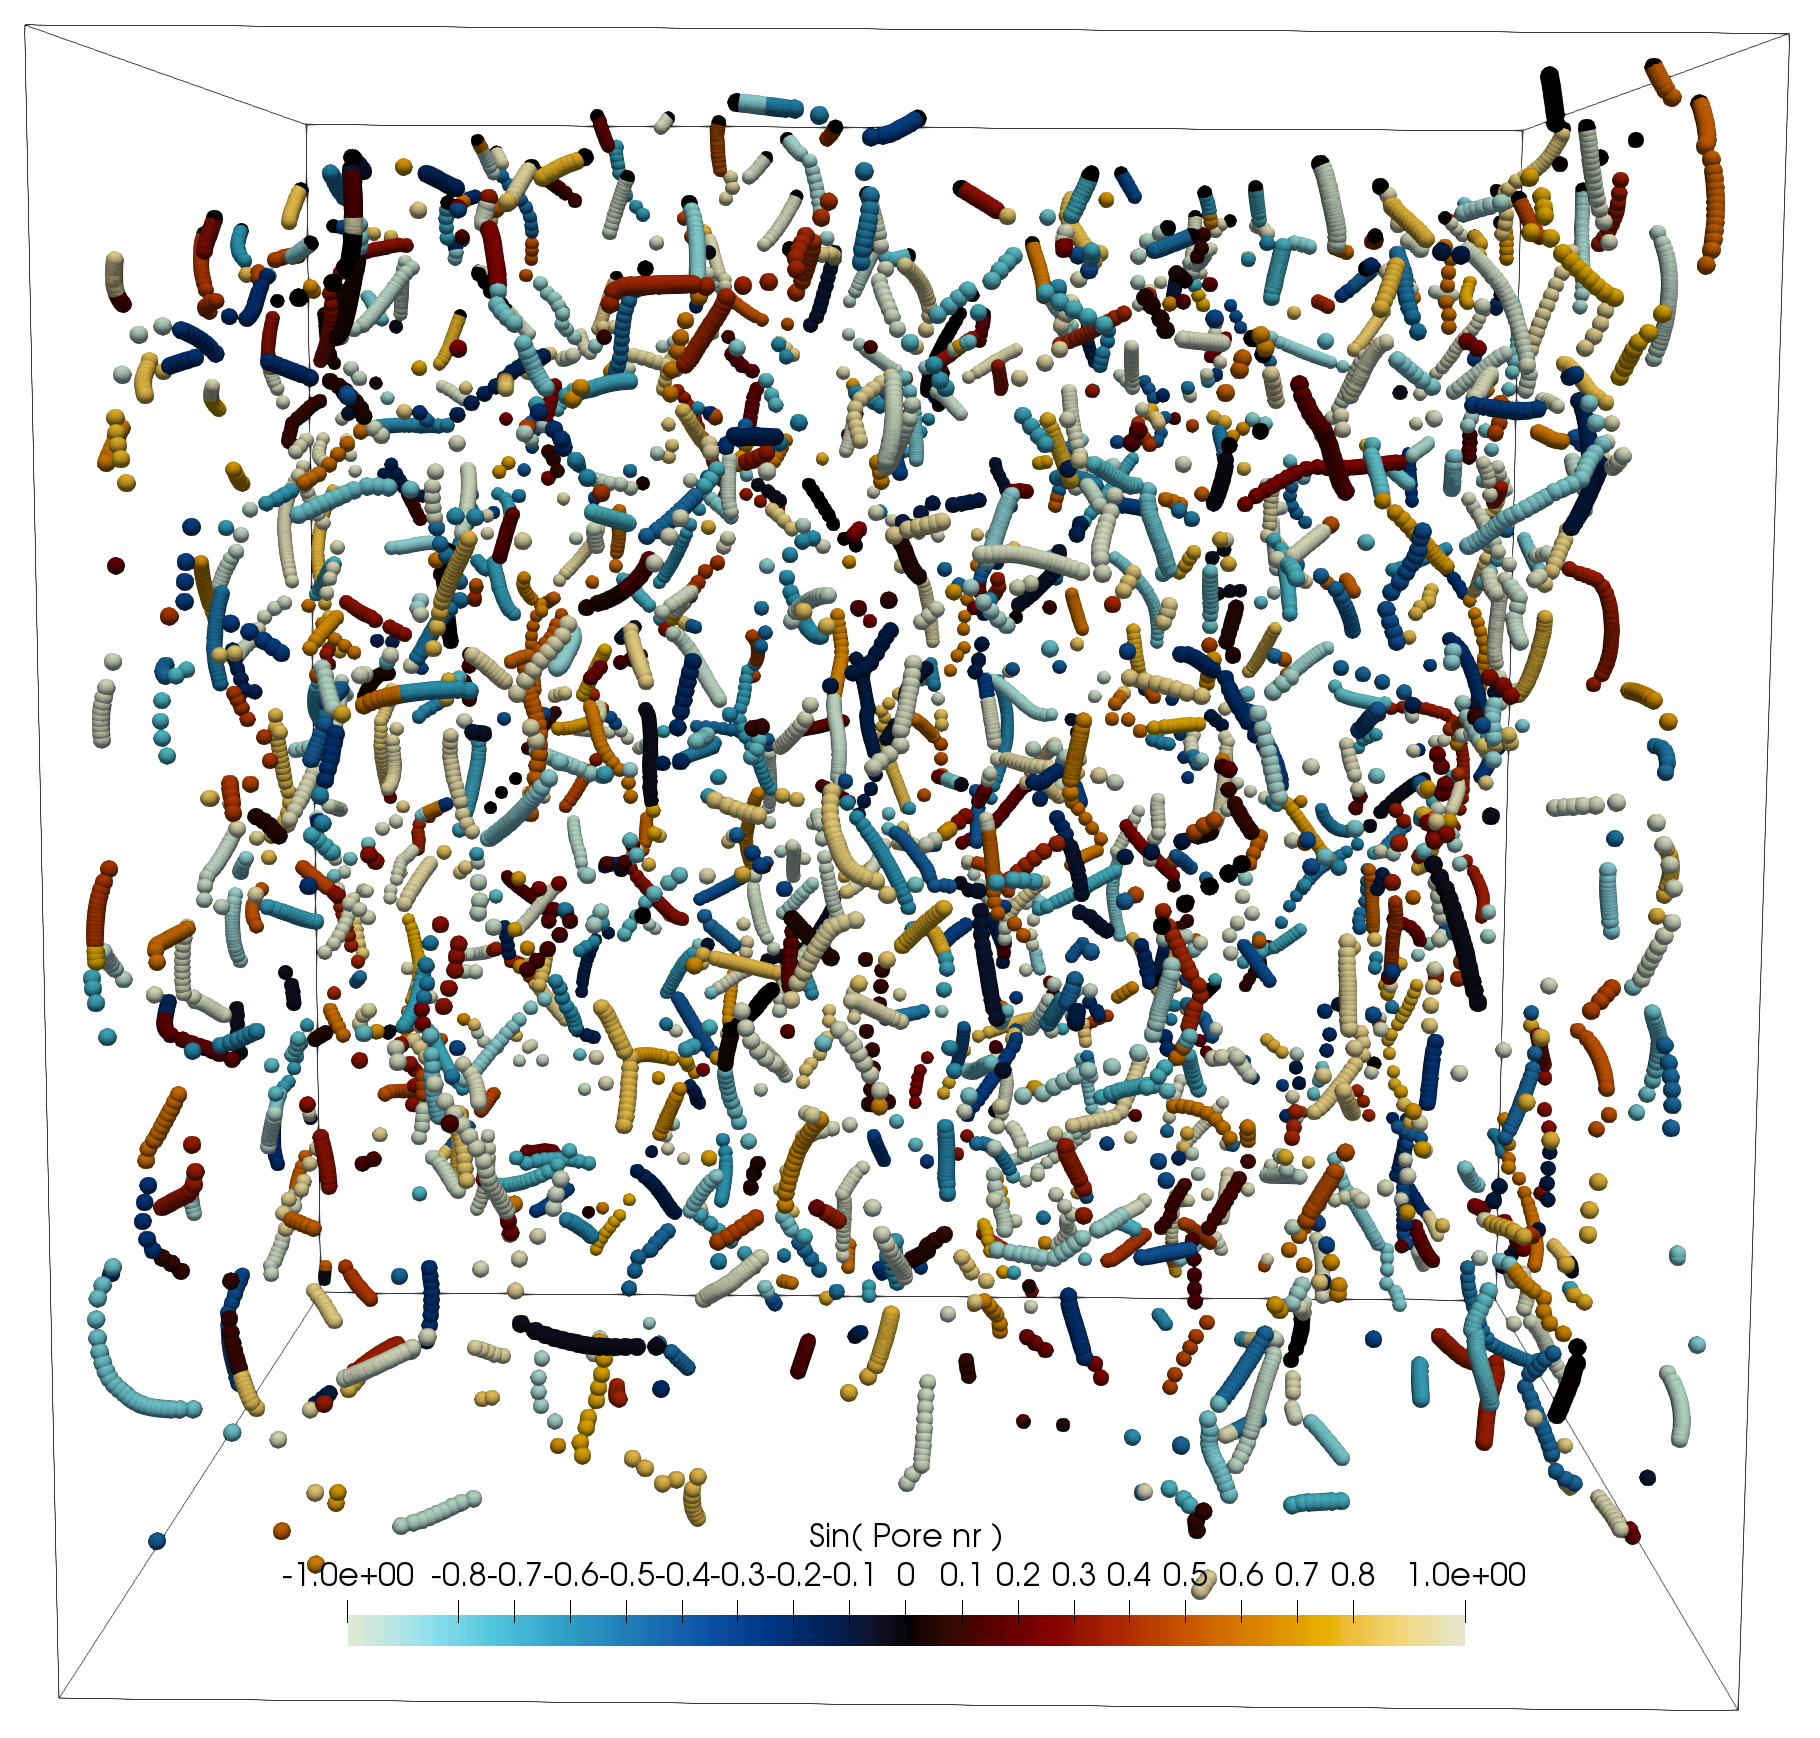
\includegraphics[height=5cm]{figures/pores_PM2.png}
\caption{Visualization of left: velocity field $|\mathbf{u}|$of an iso-pressure surface $\mathcal{S}(p)$ at pressure value $p$, middle: segmentation into iso-pressure patches  $\mathcal{S}_i(p)$, right: Pore identification throughout the porous medium. }
\end{figure}

\noindent\textbf{Extraction of pores based on iso-pressure surfaces}
Then a chain of VTK-based image analysis techniques \citeA{schroeder_visualization_2006,hernderson_paraview_2007} are employed to extract iso-pressure surfaces $\mathcal{S}(p)$ and enumerate the disconnected areas identifying as an iso-pressure slice $\mathcal{S}_i(p)$, part of a pore and measure its surface area $A_i(p)$, sphericity $\gamma_i(p)$, average location $\mathbf{x}_i(p)$ and average flux $Q_i(p)$. For each $\mathcal{S}_i(p)$ its closest neighbor $\mathcal{S}_j(p+\delta p)$ is identified by its smallest distance $d_{i,j}= \left|  \mathbf{x}_i(p)-\mathbf{x}_j(p+\delta p)\right|$. By forward integration of the first iso-pressure patches $\mathcal{S}_i(p_0)$ we identify all patches belonging to the same pore $\mathcal{P}_l(\Delta p) = \{\mathcal{S}_k(p_i)\}$. By conditioning the distances of consecutive iso pressure patches to a maximum, the ends of a pore is defined. When a splitting/merging of pores is at hand, the average position is rather sensitive, and the distance between two consecutive iso-pressure pore patches will exceed the maximum distance. Fig.~\ref{fig:segmentation} shows a visualization of the positions of the identified pores. For each $\delta p$ we can now evaluate Eq.~\ref{eq:infi_dp} and for each pore, we can evaluate Eq.~\ref{eq:R_model}. A visualization of an iso-pressure surface $\mathcal{S}(p)$ and its devision of patches is shown in Fig.\ref{fig:segmentation}. 

\noindent\textbf{Extraction of pore attributes}


\noindent\textbf{Measuring the relative Longitudinal and Transversal energy dissipation on an isopressure surface} 
In the theoretical section of the paper we have derived expressions for the longitudinal and transversal energy dissipation tensors, by 
\begin{equation}\label{eq:reduced_dissipation_tensor}
\left|\nabla_i u_j\right|^2 \approx  \left|\nabla_s u_p\right|^2 + \left|\nabla_n u_p\right|^2 .
\end{equation}
where we have assumed that the terms $ \left|\nabla_n u_n\right|^2$ and $ \left|\nabla_s u_n\right|^2$ are negligible. We will show two examples where we have calculated the individual terms of the total viscous dissipation. Because the highest dissipation is expected to be located near the porous media interface and the discretization also refined at the interface the numerical noise is also expected to be higher, see Fig\ref{fig:numerical noise}. All 3 porous media contain some points in the mesh where the VTK gradient filter can't factorize the linear system which leads to very high values of the respected fields. The origin lies likely in the mesh quality generated by the snappyHexMesh generator contained in the openFoam simulation. Since the simulations have all converged we do not question the original simulation results but we do note that post-processing of these meshes can be difficult especially if gradients have to be calculated. Nevertheless we have tried to quantify the relevance of the transversal and longitudinal terms of the viscous dissipation tensor. We have chosen to threshold the unreasonable high gradient terms based on outliers in the histograms of the gradients. For the first porous media the porous media the refinement was chosen a degree higher than the others, and led to `nan' results of the integrated relative contributions. For the two other porous media we have found reasonable results given in Table \ref{tab:sm1}. Since we have to filter out quit some data that exhibits unreasonable high values the percentages are not adding up to $100\%$. By visual inspection we can examine the term $\left|\nabla_i u_j\right|^2$ in all porous media and we see that the total dissipation correlates with gradients in the transverse direction. Also in this data we can see that for Porous Media 3 the relative contribution of the longitudinal term $ \left|\nabla_n u_p\right|^2$, $24\%$ is in the same order as the transversal term $ \left|\nabla_s u_p\right|^2$ which amounts to $32\%$. This observation is in agreement with the fitting of the two contributions in the paper.


\end{article}

\begin{table}[htbp!]\label{tab:sm1}
\centering
\begin{tabular}{l|c|c|c|c|c}
PM & & $\left|\nabla_s u_p\right|^2$ & $ \left|\nabla_n u_p\right|^2$ & $\left|\nabla_n u_n\right|^2$ & $\left|\nabla_n u_n\right|^2$ \\
\hline
PM2 &  & $71 \%$ & $17\%$ & $12\%$ & $12\%$ \\
PM3 &  & $32 \%$ & $24\%$ & $10\%$ & $5\%$ \\
\end{tabular}
\caption{\label{tab:table-name}Estimated relative contributions to the total viscous dissipation on an iso-pressure surface. }
\end{table}




\begin{figure}
\setfigurenum{S1} %%You can change number for each figure if you want, not required. "S" prepended automatically.
\noindent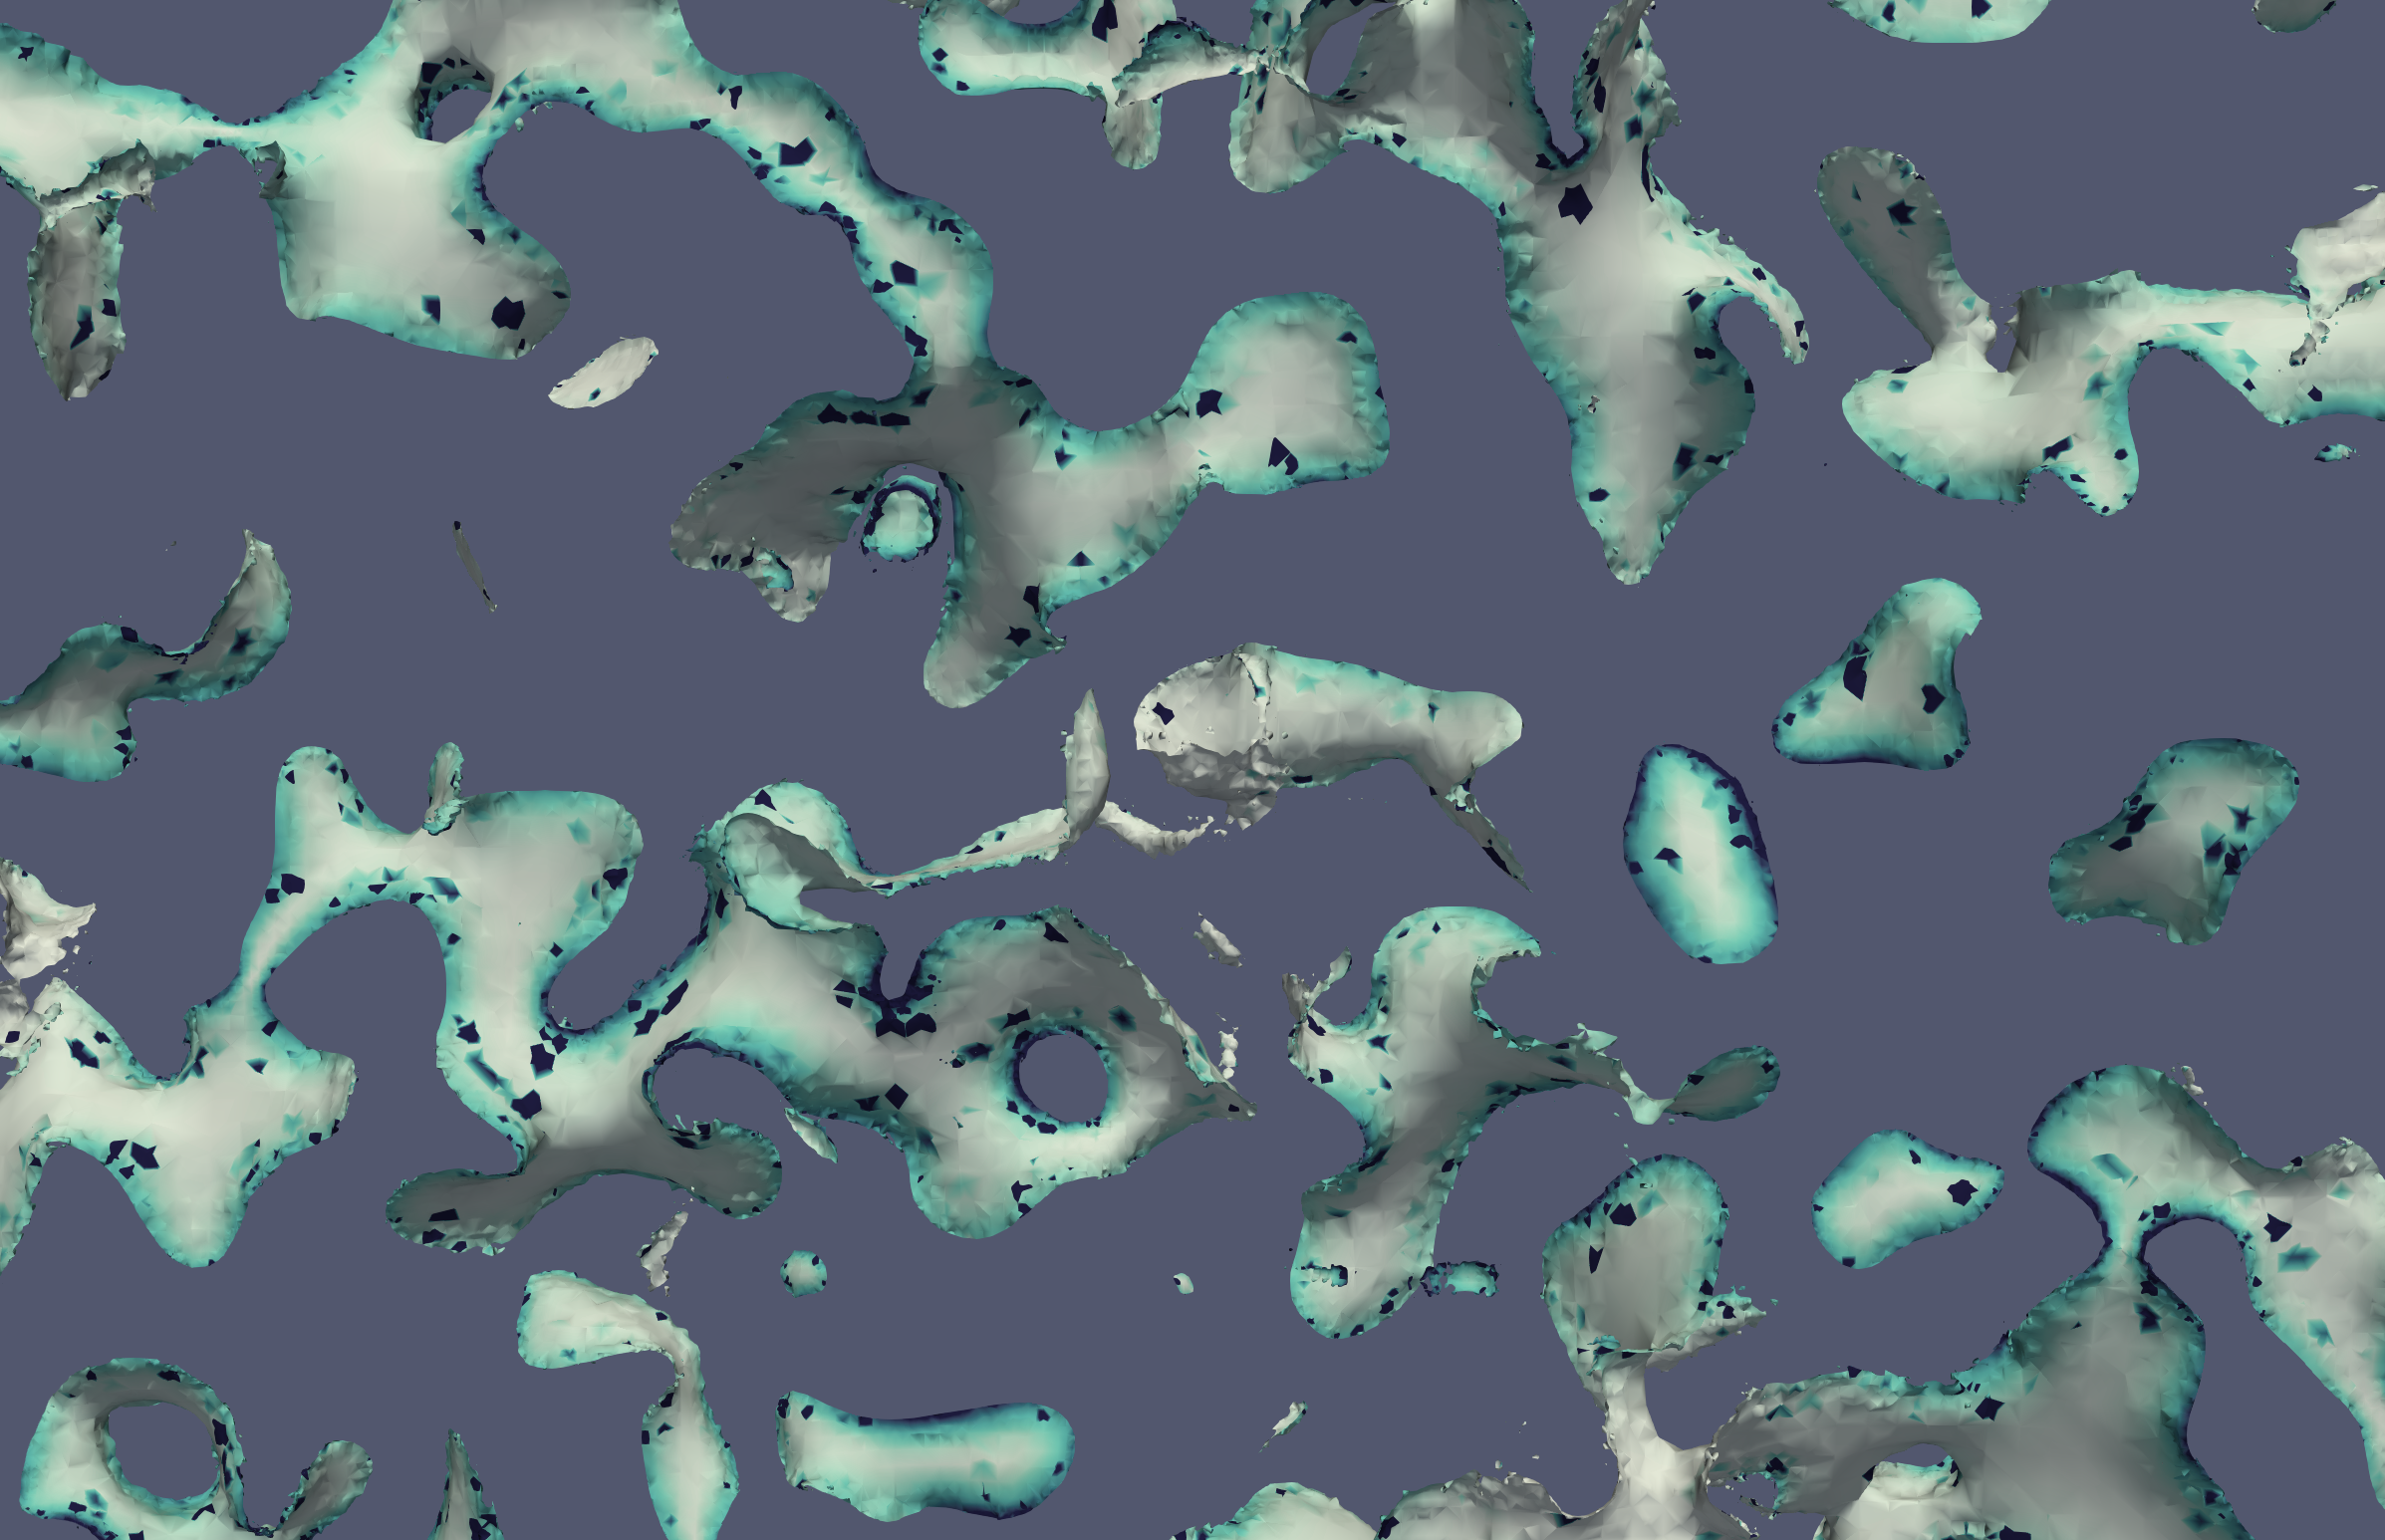
\includegraphics[height=8cm]{figures/nummeric_noise.png}
\caption{A visualization of the energy dissipation tensor $|\mathbf{\nabla}\otimes \mathbf{u}|$ on a iso-pressure surface of PM1, indicating the numerical issues}
\label{fig:numerical noise}
\end{figure}

\bibliography{library.bib}

% Copy/paste for multiples of each file type as needed.

% enter figures and tables below here: %%%%%%%
%
%
%
%
% EXAMPLE FIGURES
% ---------------
% If you get an error about an unknown bounding box, try specifying the width and height of the figure with the natwidth and natheight options.
% \begin{figure}
%\setfigurenum{S1} %%You can change number for each figure if you want, not required. "S" prepended automatically.
% \noindent\includegraphics[natwidth=800px,natheight=600px]{samplefigure.eps}
%\caption{caption}
%\label{epsfiguresample}
%\end{figure}
%
%
% Giving latex a width will help it to scale the figure properly. A simple trick is to use \textwidth. Try this if large figures run off the side of the page.
% \begin{figure}
% \noindent\includegraphics[width=\textwidth]{anothersample.png}
%\caption{caption}
%\label{pngfiguresample}
%\end{figure}
%
%
%\begin{figure}
%\noindent\includegraphics[width=\textwidth]{athirdsample.pdf}
%\caption{A pdf test figure}
%\label{pdffiguresample}
%\end{figure}
%
% PDFLatex does not seem to be able to process EPS figures. You may want to try the epstopdf package.
%
%
% ---------------
% EXAMPLE TABLE
%
%\begin{table}
%\settablenum{S1} %%Change number for each table
%\caption{Time of the Transition Between Phase 1 and Phase 2\tablenotemark{a}}
%\centering
%\begin{tabular}{l c}
%\hline
% Run  & Time (min)  \\
%\hline
%  $l1$  & 260   \\
%  $l2$  & 300   \\
%  $l3$  & 340   \\
%  $h1$  & 270   \\
%  $h2$  & 250   \\
%  $h3$  & 380   \\
%  $r1$  & 370   \\
%  $r2$  & 390   \\
%\hline
%\end{tabular}
%\tablenotetext{a}{Footnote text here.}
%\end{table}
% ---------------
%
% EXAMPLE LARGE TABLE (UPLOADED SEPARATELY)
%\begin{table}
%\settablenum{S1} %%Change number for each table
%\caption{Time of the Transition Between Phase 1 and Phase 2\tablenotemark{a}}
%\end{table}


\end{document}

%%%%%%%%%%%%%%%%%%%%%%%%%%%%%%%%%%%%%%%%%%%%%%%%%%%%%%%%%%%%%%%

More Information and Advice:

%% ------------------------------------------------------------------------ %%
%
%  SECTION HEADS
%
%% ------------------------------------------------------------------------ %%

% Capitalize the first letter of each word (except for
% prepositions, conjunctions, and articles that are
% three or fewer letters).

% AGU follows standard outline style; therefore, there cannot be a section 1 without
% a section 2, or a section 2.3.1 without a section 2.3.2.
% Please make sure your section numbers are balanced.
% ---------------
% Level 1 head
%
% Use the \section{} command to identify level 1 heads;
% type the appropriate head wording between the curly
% brackets, as shown below.
%
%An example:
%\section{Level 1 Head: Introduction}
%
% ---------------
% Level 2 head
%
% Use the \subsection{} command to identify level 2 heads.
%An example:
%\subsection{Level 2 Head}
%
% ---------------
% Level 3 head
%
% Use the \subsubsection{} command to identify level 3 heads
%An example:
%\subsubsection{Level 3 Head}
%
%---------------
% Level 4 head
%
% Use the \subsubsubsection{} command to identify level 3 heads
% An example:
%\subsubsubsection{Level 4 Head} An example.
%
%% ------------------------------------------------------------------------ %%
%
%  IN-TEXT LISTS
%
%% ------------------------------------------------------------------------ %%
%
% Do not use bulleted lists; enumerated lists are okay.
% \begin{enumerate}
% \item
% \item
% \item
% \end{enumerate}
%
%% ------------------------------------------------------------------------ %%
%
%  EQUATIONS
%
%% ------------------------------------------------------------------------ %%

% Single-line equations are centered.
% Equation arrays will appear left-aligned.

Math coded inside display math mode \[ ...\]
 will not be numbered, e.g.,:
 \[ x^2=y^2 + z^2\]

 Math coded inside \begin{equation} and \end{equation} will
 be automatically numbered, e.g.,:
 \begin{equation}
 x^2=y^2 + z^2
 \end{equation}

% IF YOU HAVE MULTI-LINE EQUATIONS, PLEASE
% BREAK THE EQUATIONS INTO TWO OR MORE LINES
% OF SINGLE COLUMN WIDTH (20 pc, 8.3 cm)
% using double backslashes (\\).

% To create multiline equations, use the
% \begin{eqnarray} and \end{eqnarray} environment
% as demonstrated below.
\begin{eqnarray}
  x_{1} & = & (x - x_{0}) \cos \Theta \nonumber \\
        && + (y - y_{0}) \sin \Theta  \nonumber \\
  y_{1} & = & -(x - x_{0}) \sin \Theta \nonumber \\
        && + (y - y_{0}) \cos \Theta.
\end{eqnarray}

%If you don't want an equation number, use the star form:
%\begin{eqnarray*}...\end{eqnarray*}

% Break each line at a sign of operation
% (+, -, etc.) if possible, with the sign of operation
% on the new line.

% Indent second and subsequent lines to align with
% the first character following the equal sign on the
% first line.

% Use an \hspace{} command to insert horizontal space
% into your equation if necessary. Place an appropriate
% unit of measure between the curly braces, e.g.
% \hspace{1in}; you may have to experiment to achieve
% the correct amount of space.


%% ------------------------------------------------------------------------ %%
%
%  EQUATION NUMBERING: COUNTER
%
%% ------------------------------------------------------------------------ %%

% You may change equation numbering by resetting
% the equation counter or by explicitly numbering
% an equation.

% To explicitly number an equation, type \eqnum{}
% (with the desired number between the brackets)
% after the \begin{equation} or \begin{eqnarray}
% command.  The \eqnum{} command will affect only
% the equation it appears with; LaTeX will number
% any equations appearing later in the manuscript
% according to the equation counter.
%

% If you have a multiline equation that needs only
% one equation number, use a \nonumber command in
% front of the double backslashes (\\) as shown in
% the multiline equation above.

%% ------------------------------------------------------------------------ %%
%
%  SIDEWAYS FIGURE AND TABLE EXAMPLES
%
%% ------------------------------------------------------------------------ %%
%
% For tables and figures, add \usepackage{rotating} to the paper and add the rotating.sty file to the folder.
% AGU prefers the use of {sidewaystable} over {landscapetable} as it causes fewer problems.
%
% \begin{sidewaysfigure}
% \includegraphics[width=20pc]{samplefigure.eps}
% \caption{caption here}
% \label{label_here}
% \end{sidewaysfigure}
%
%
%
% \begin{sidewaystable}
% \caption{}
% \begin{tabular}
% Table layout here.
% \end{tabular}
% \end{sidewaystable}
%
%

